\documentclass{beamer}
\usepackage{apacite}
\usepackage{caption}
\usepackage[font=small, labelfont=bf]{subcaption}
\usepackage{textpos}
\usetheme{Darmstadt}
\usepackage{graphicx}
\usepackage{float}
%packages for definitions%%%%%%%%%%%%%%
\usepackage{blindtext}
\usepackage{scrextend}
\usepackage{amsmath}
\addtokomafont{labelinglabel}{\sffamily}
\usepackage{tikz}
    \usetikzlibrary{shapes}
    \usetikzlibrary{positioning}
    \usetikzlibrary{arrows}
    \usetikzlibrary{fit}
    \usetikzlibrary{decorations.pathreplacing}
    \usetikzlibrary{shadows.blur}
    \usetikzlibrary{shapes.symbols}

\newcommand\FourQuad[4]{%
    \begin{minipage}[b][.35\textheight][t]{.47\textwidth}#1\end{minipage}\hfill%
    \begin{minipage}[b][.35\textheight][t]{.47\textwidth}#2\end{minipage}\\[0.5em]
    \begin{minipage}[b][.35\textheight][t]{.47\textwidth}#3\end{minipage}\hfill
    \begin{minipage}[b][.35\textheight][t]{.47\textwidth}#4\end{minipage}%
}

%%%%%%%%%%%%%%%%%%%%%%%%%%%%%%%%%%%%%%%
\AtBeginSection[]{
    \begin{frame}
    \vfill
    \centering
    \begin{beamercolorbox}[sep=8pt,center,shadow=true,rounded=true]{title}
        \usebeamerfont{title}\insertsectionhead\par%
    \end{beamercolorbox}
    \vfill
    \end{frame}
}
\title{A Neural Algorithm of Artistic Style \\ { \tiny Leon A. Gatys, Alexander S. Ecker, Matthias Bethge}}
\author{Behnam Rasoolian, Christian Kauten}
\institute{Auburn University}
\definecolor{auburn_orange}{RGB}{221, 85, 12}
\definecolor{auburn_blue}{RGB}{3, 36, 77}
\date{}
\begin{document}
\tikzset{
    mystyle/.style={
    inner sep=0pt,
    minimum width = .5cm,
    minimum height = .5cm,
    text width=1cm,
    circle,
    draw=black,
    align=center,
  }
}
\tikzset{
    myEdgeStyle/.style={
    ->,
    line width = 1pt
    %ultra thick
  }
}
\tikzset{
    myArrow/.style={
    single arrow,
    draw,
    text width =.3cm,
    scale=.8,
    shade, shading=axis, left color=orange, right color=yellow,
        shading angle=45,
    blur shadow={shadow blur steps=5,shadow blur extra rounding=1.3pt}
}
}

\frame{\titlepage}

\begin{frame}{Notations}
    \begin{itemize}
        \item $\mathbf{p}$: The original, content image
        \item $\mathbf{a}$: The original, artwork image
        \item $\mathbf{x}$: The image to be generated. It is initiated as a
            random noise image.
        \item $F^l$: \textbf{Feature Map} at level l, is the result of appling
            filters at level $l$. If $N_l$ filters are applier at level $l$,
            then this feature map has a depth of $N_l$.
        \item $N_l$: The number of filters applier at level $l$. This is
            the same as the depts of the feature map at level
            $l$.
        \item $M_l$: the dimension of the feature map at level l, which
            is equal to $N_l \times M_l$.
        \item $\mathbf{F}^l$: The feature map at level $l$. it is an
            $N_l \times M_l$ matrix.
    \end{itemize}
\end{frame}

\begin{frame}{Notations}
    \begin{figure}[H]
        \centering
        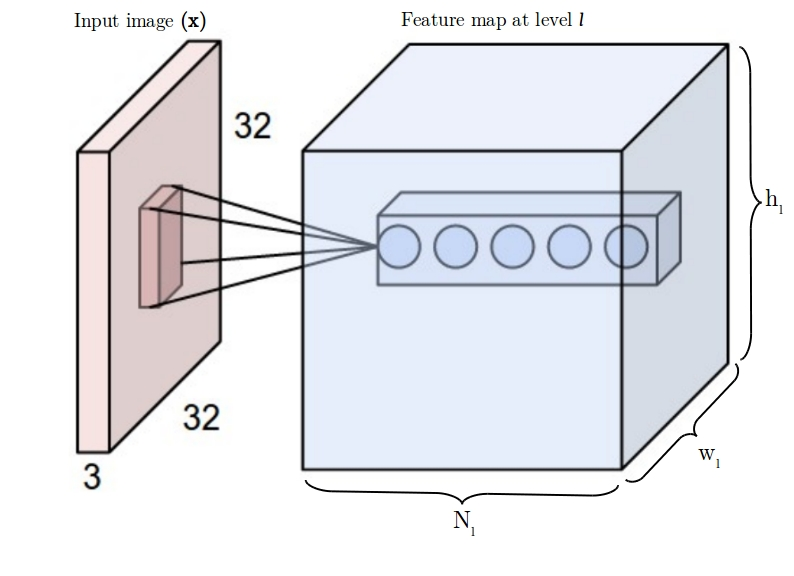
\includegraphics[width=.8\textwidth]{img/levels.jpg}
    \end{figure}
\end{frame}

\begin{frame}{Content Representation}
    \begin{itemize}
        \item Gradient descent is performed on a white noise image
            ($\mathbf{x}$) and a content image
            ($\mathbf{p}$)
        \item $F^l$ and $P^l$: Respective feature maps of the
            noise image and the original image
        \item Goal: Reduce the squared-error loss between $F^l$ and $P^l$.
    \begin{equation}
        \mathcal{L}(\mathbf{p}, \mathbf{x}, l) =
        \frac{1}{2} \sum_{i=1}^{N_l}\sum_{j=1}^{M_l}{(F^l_{ij} - P^l_{ij})^2}
    \end{equation}
    \end{itemize}
\end{frame}

\begin{frame}{Content Representation}
    The gradient of this loss with respect to activations in $l$ can be easily
    calculated:
    \begin{equation}
        \frac{\partial \mathcal{L}_{content}}{\partial F^l_{ij}}
        =
        \begin{cases}
            (F^l - P^l)_{ij} & \iff F^l_{ij} > 0 \\
            0 & \iff F^l_{ij} < 0 \\
        \end{cases}
    \end{equation}
\end{frame}

\begin{frame}{Content Reconstruction}
\begin{figure}[ht]
    \begin{minipage}[b]{0.45\linewidth}
        \centering
        \caption{white noise image $\mathbf{x}$}
        
\includegraphics[width=\textwidth]{img/content/noise.png}
    \end{minipage}
    \hspace{0.5cm}
    \begin{minipage}[b]{0.45\linewidth}
        \centering
        \caption{content image $\mathbf{p}$}
        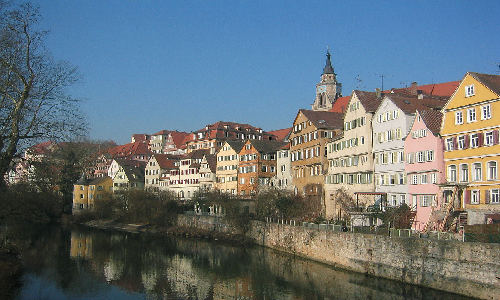
\includegraphics[width=\textwidth]{img/content/tubingen.png}
    \end{minipage}
\end{figure}
\end{frame}

\begin{frame}{Content Reconstruction}
\begin{figure}[ht]
\centering
\caption{Block 1 Conv 1}
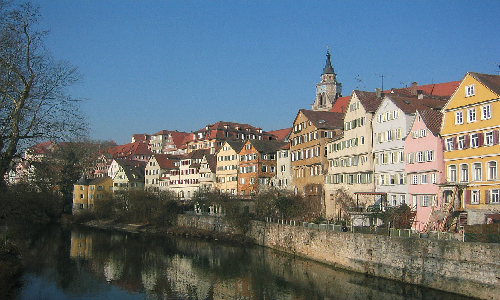
\includegraphics[width=\textwidth]{img/content/block1_conv1.png}
\end{figure}
\end{frame}

\begin{frame}{Content Reconstruction}
\begin{figure}[ht]
\centering
\caption{Block 2 Conv 1}
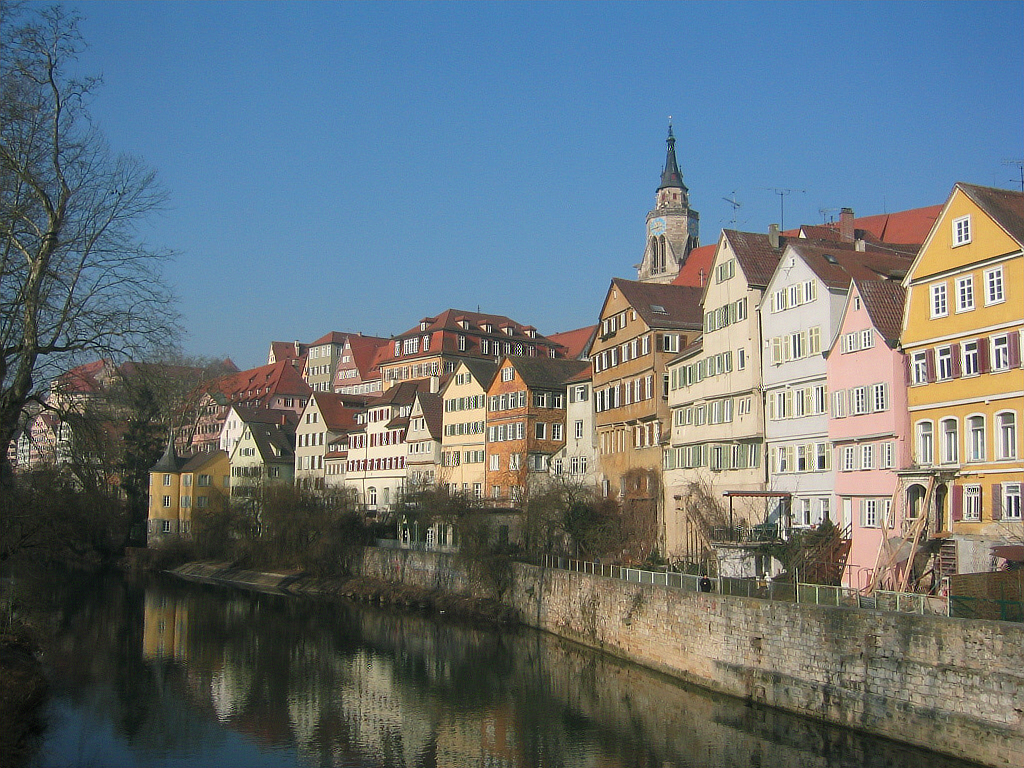
\includegraphics[width=\textwidth]{img/content/block2_conv1.png}
\end{figure}
\end{frame}

\begin{frame}{Content Reconstruction}
\begin{figure}[ht]
\centering
\caption{Block 3 Conv 1}
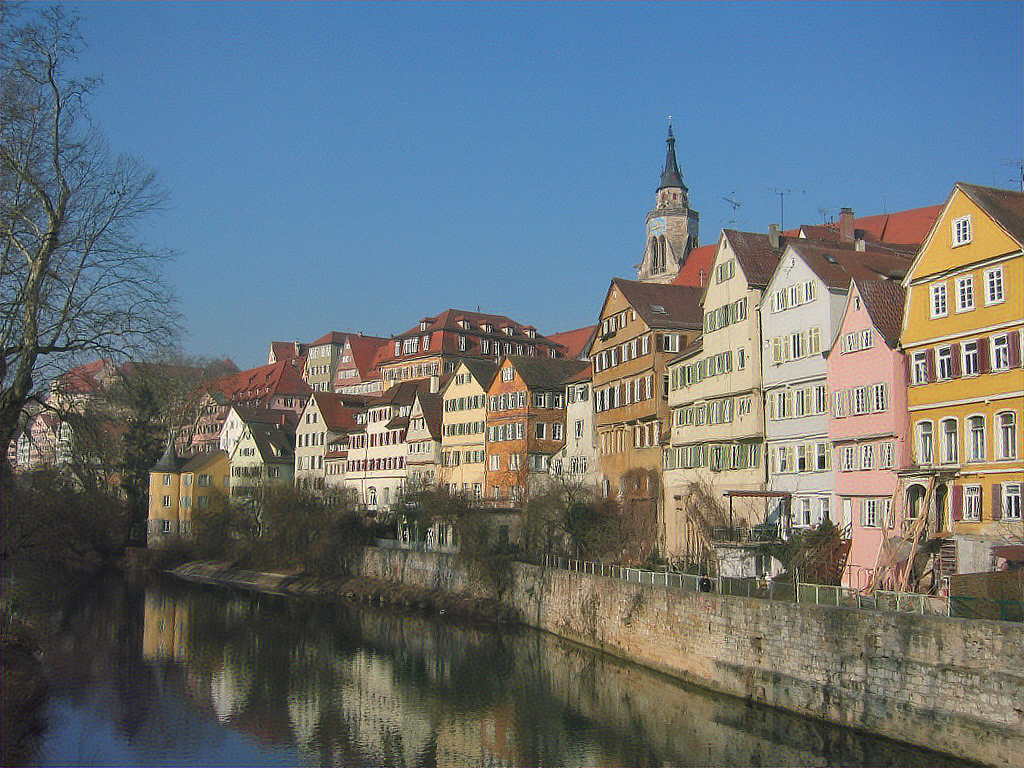
\includegraphics[width=\textwidth]{img/content/block3_conv1.png}
\end{figure}
\end{frame}

\begin{frame}{Content Reconstruction}
\begin{figure}[ht]
\centering
\caption{Block 4 Conv 1}
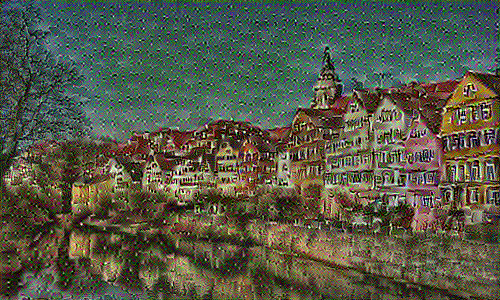
\includegraphics[width=\textwidth]{img/content/block4_conv1.png}
\end{figure}
\end{frame}

\begin{frame}{Content Reconstruction}
\begin{figure}[ht]
\centering
\caption{Block 5 Conv 1}
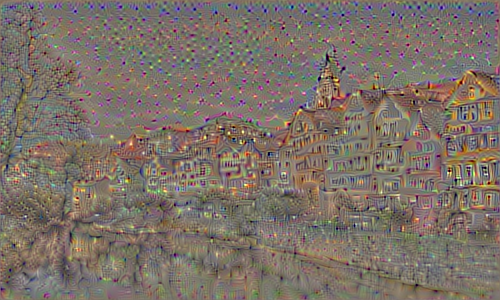
\includegraphics[width=\textwidth]{img/content/block5_conv1.png}
\end{figure}
\end{frame}

\begin{frame}{Style Representation}
Style representation is achived via the ``Gram Matrix'' $G$. Gram matrix is
an $N_l \times N_l$ matrix which calculates the correlations between
different filter responses.

\begin{equation}
    \mathbf{G^l}_{ij} = \mathbf{{F^l}^T}_i \times \mathbf{F^l}_j
    = (\mathbf{{F^l}^T} \times \mathbf{F^l})_{ij}
\end{equation}
\end{frame}

\begin{frame}{Style Representation}
Given $G^l$ and $A^l$ as respective Gram matrices of the
noise image and the original image, our goal is to reduce the overal difference
between $G^l$ and $A^l$. In ths sense,
Contribution of layer $l$ to the total loss is
\begin{equation}
    E_l = \frac{1}{4N_l^2M_l^2} \sum_{i}^{N_l}\sum_{j}^{N_l}{(G^l_{ij} - A^l_{ij})^2}
    = \mathbf{1}^T(\mathbf{G} - \mathbf{A})(\mathbf{G} - \mathbf{A})^T
\end{equation}
\end{frame}

\begin{frame}{Style Representation}
The total style loss is:
\begin{equation}
    \mathcal{L}_{style}(\mathbf{a}, \mathbf{x}) = \sum_{l=0}^L {w_l E_l }
\end{equation}
\begin{equation}
    \frac{\partial \mathcal{L}_{style}}{\partial F^l_{ij}} = \frac{\partial E_l}{\partial F^l_{ij}} =
    (4(\mathbf{G}^l - \mathbf{A}^l) \times \mathbf{F}^l)_{ij}
\end{equation}
\end{frame}

\begin{frame}{Style Representation}
\begin{equation}
    \frac{\partial \mathcal{L}_{style}}{\partial F^l_{ij}} = \frac{\partial E_l}{\partial F^l_{ij}} =
    (4(\mathbf{G}^l - \mathbf{A}^l) \times \mathbf{F}^l)_{ij}
\end{equation}
    \begin{figure}
    \begin{tikzpicture}[scale=.84, every node/.style={scale=.7}, transform shape]
        \node (a) at (-5, 0) {};
        \node [mystyle] (b) [right=2cm of a] {$ \times X^T$};
        \draw [myEdgeStyle] (a.east) to  node [auto] (ab) {$\mathbf{F^l}_{N_l \times M_l}$}(b.west);
        \draw [myEdgeStyle] (a.east) to  node [red] [below] (ab) {$2(\mathbf{G} - \mathbf{A}) \times 2\mathbf{F}$}(b.west);
        \node [mystyle, ellipse, text height = .5cm, text width = 2cm] (c) [right=2cm of b] {$ (\mathbf{X} - \mathbf{A}_l)^2$};
        \draw [myEdgeStyle] (b.east) to node [auto] (bc) {$\mathbf{G}_{N_l \times N_l}$} (c.west) ;
        \draw [myEdgeStyle] (b.east) to node  [red][below] (bc) {$2(\mathbf{G} - \mathbf{A})_{N_l \times N_l}$} (c.west) ;
        \node [mystyle] (d) [right=2cm of c] {$\times$};
        \draw [myEdgeStyle] (c.east) to node [auto] (cd) {$(G - A)^2_{N_l \times N_l}$} (d.west) ;
        \draw [myEdgeStyle] (c.east) to node  [red][below] (cd) {$1_{N_l \times N_l}$} (d.west) ;
        \node (bcd) [below=1cm of cd] {};
        \draw [myEdgeStyle] (bcd.east) -| node [above left= .1and .4cm] {$\mathbf{1}_{N_l \times 1}$} (d.south) ;
        \node [mystyle] (e) [right=2cm of d] {$\times$};
        \draw [myEdgeStyle] (d.east) to node [above] (de) {$E'_{N_l \times 1}$} (e.west) ;
        \draw [myEdgeStyle] (d.east) to node  [red][below] (de) {$\mathbf{1}_{N_l \times 1}$} (e.west) ;
        \node (bde) [below=1cm of de] {};
        \draw [myEdgeStyle] (bde.east) -| node [above left= .1and .4cm] {$\mathbf{1}^T_{1 \times N_l}$} (e.south) ;
        \node (f) [right=1.5cm of e] {};
        \draw [myEdgeStyle] (e.east) to node [auto] (ef) {$E$} (f.west) ;
        \draw [myEdgeStyle] (e.east) to node  [red][below] (ef2) {$1$} (f.west) ;
    \end{tikzpicture}
    \end{figure}
\end{frame}

\begin{frame}{Style Reconstruction}
\begin{figure}[ht]
    \begin{minipage}[b]{0.45\linewidth}
        \centering
        \caption{white noise image $\mathbf{x}$}
        
\includegraphics[width=\textwidth]{img/style/noise.png}
    \end{minipage}
    \hspace{0.5cm}
    \begin{minipage}[b]{0.45\linewidth}
        \centering
        \caption{artwork image $\mathbf{a}$}
        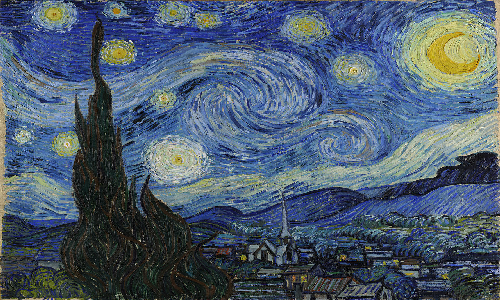
\includegraphics[width=\textwidth]{img/style/starry_night.png}
    \end{minipage}
\end{figure}
\end{frame}

\begin{frame}{Style Reconstruction}
\begin{figure}[ht]
\centering
\caption{Conv 1 of Block 1}
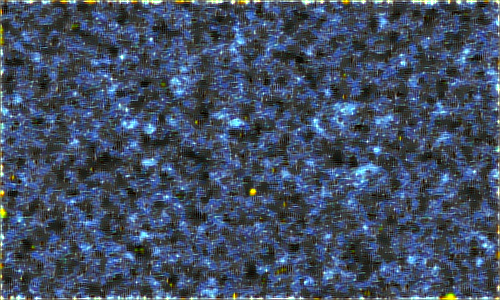
\includegraphics[width=\textwidth]{img/style/block1_conv1.png}
\end{figure}
\end{frame}

\begin{frame}{Style Reconstruction}
\begin{figure}[ht]
\centering
\caption{Conv 1 of Block 1, 2}
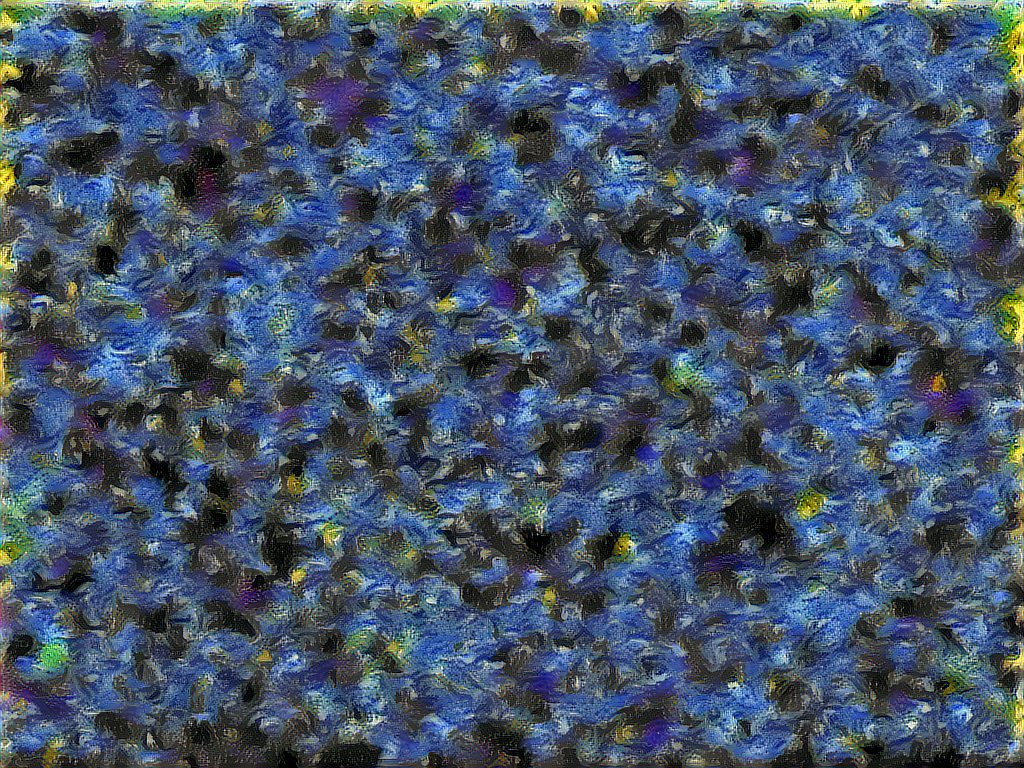
\includegraphics[width=\textwidth]{img/style/block2_conv1.png}
\end{figure}
\end{frame}

\begin{frame}{Style Reconstruction}
\begin{figure}[ht]
\centering
\caption{Conv 1 of Block 1, 2, 3}
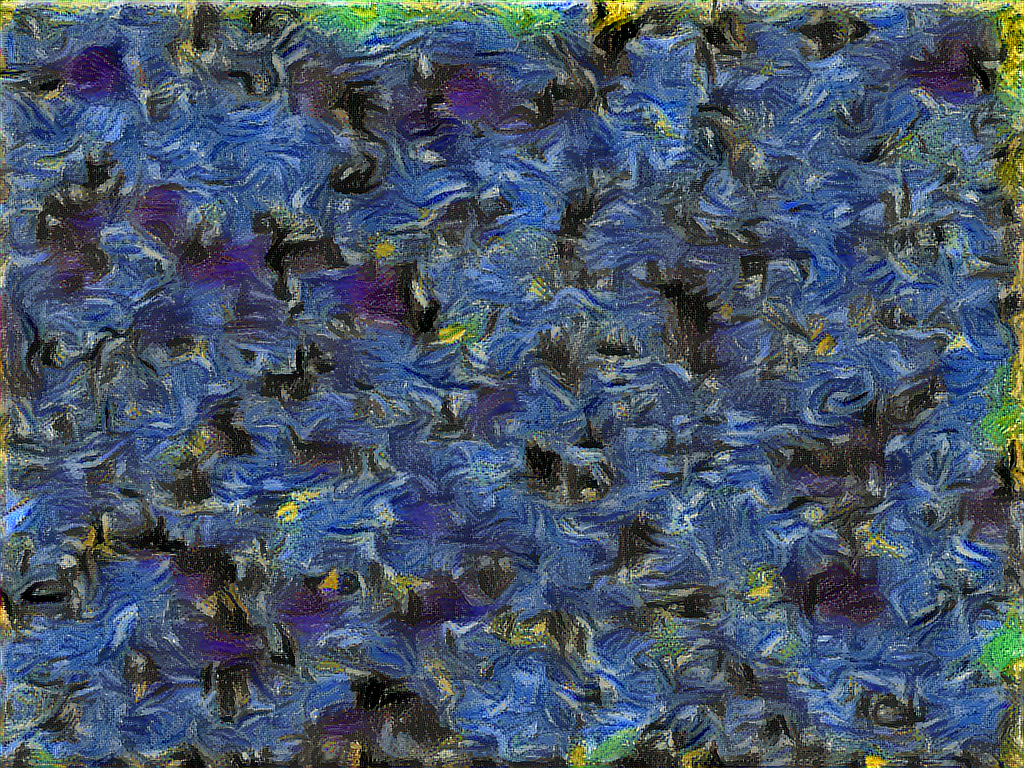
\includegraphics[width=\textwidth]{img/style/block3_conv1.png}
\end{figure}
\end{frame}

\begin{frame}{Style Reconstruction}
\begin{figure}[ht]
\centering
\caption{Conv 1 of Block 1, 2, 3, 4}
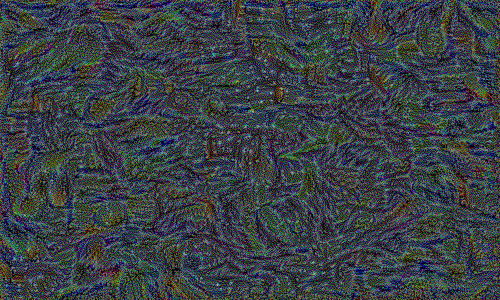
\includegraphics[width=\textwidth]{img/style/block4_conv1.png}
\end{figure}
\end{frame}

\begin{frame}{Style Reconstruction}
\begin{figure}[ht]
\centering
\caption{Conv 1 of Block 1, 2, 3, 4, 5}
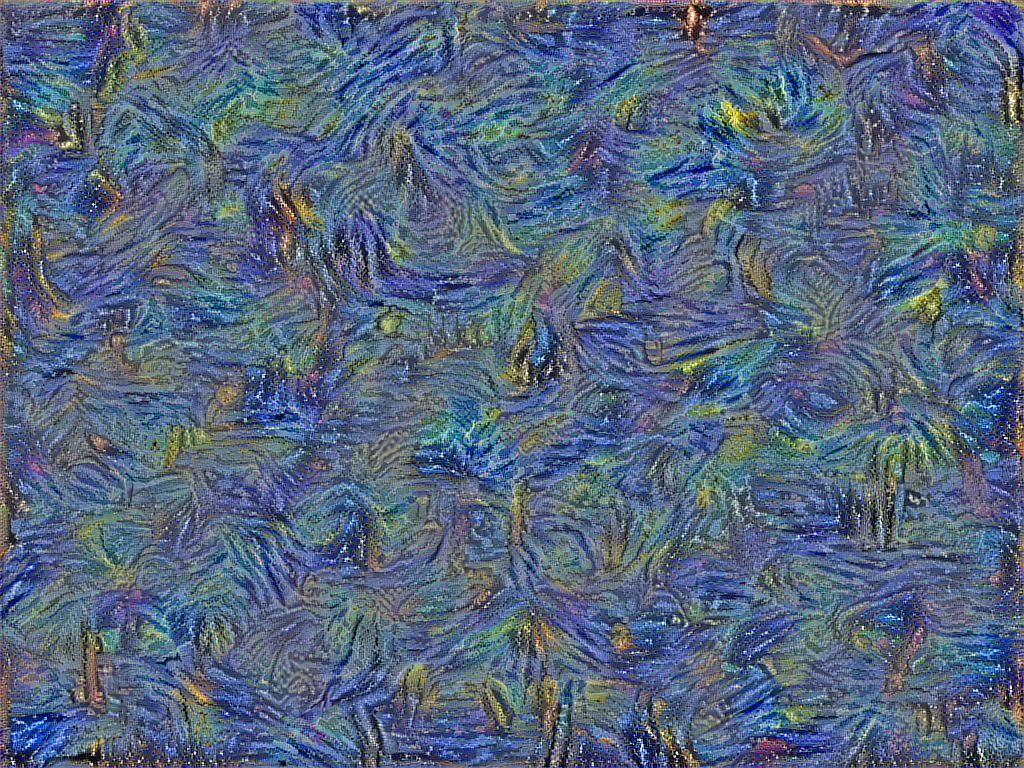
\includegraphics[width=\textwidth]{img/style/block5_conv1.png}
\end{figure}
\end{frame}

\begin{frame}{Style Transfer}
\FourQuad{
    \begin{figure}[ht]
    \centering
    \caption{Shipwreck}
    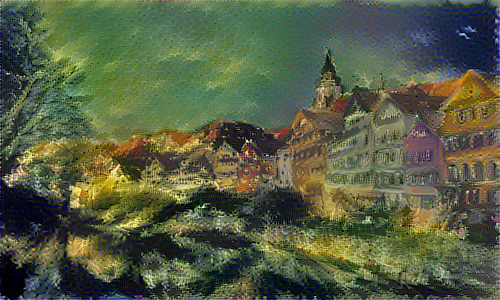
\includegraphics[width=0.8\textwidth]{img/transfer/shipwreck}
    \end{figure}
}{
\vfill
    \begin{figure}[ht]
    \centering
    \caption{Starry Starry Night}
    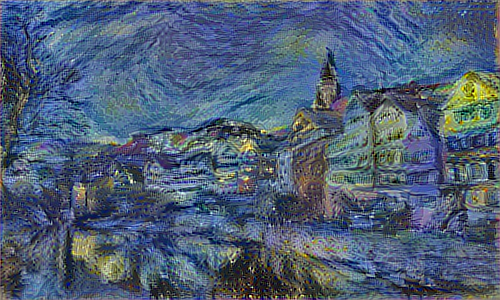
\includegraphics[width=0.8\textwidth]{img/transfer/starry-starry-night}
    \end{figure}
}{
    \begin{figure}[ht]
    \centering
    \caption{Seated Nudes}
    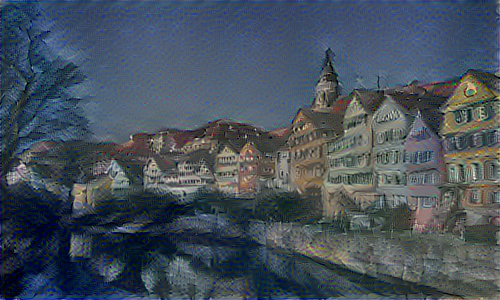
\includegraphics[width=0.8\textwidth]{img/transfer/seated-nudes}
    \end{figure}
}{
    \begin{figure}[ht]
    \centering
    \caption{Scream}
    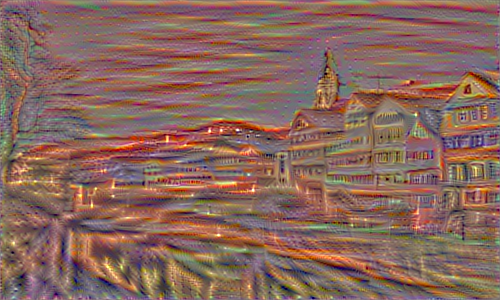
\includegraphics[width=0.8\textwidth]{img/transfer/scream}
    \end{figure}
}
\end{frame}


\end{document}
